\section{MODEL DATA}
\subsection{Priority Data}
\begin{frame}{MODEL DATA}
\framesubtitle{Priority Data}
\begin{multicols}{2}
    \begin{table}[H]
    \centering
    \begin{tabular}{lp{4cm}}
    \hline
    \textbf{ID} & \textbf{Name}                                       \\ \hline
    3           & General Pharmacy                                    \\
    4           & Appointment confirmation \& PAC, MP and policy SURA \\
    5           & Procedure after appointment                                             \\
    7           & Preferential Pharmacy                               \\
    8           & Pharmacy PAC, MP y SURA policy                      \\
    9           & Preferential Appointment confirmation 
             \\
    10       & Scheduled retrieval    
    \\ \hline
    \end{tabular}
    \caption{Types of services}
    \label{tab:types_serv}
    \end{table}
    \columnbreak
    \begin{table}[H]
\centering
\begin{tabular}{ccl}
\hline
\textbf{Set} & \textbf{Amount} & \textbf{Priority} \\ \hline
1            & 1               & {[}10{]}          \\ 
2            & 1               & {[}4, 9, 5{]}     \\
3            & 1               & {[}4, 5, 9{]}     \\
4            & 2               & {[}7, 3, 8, 10{]} \\
5            & 4               & {[}3, 8, 7, 10{]} \\
6            & 5               & {[}3, 7, 8, 10{]} \\
\hline
\end{tabular}
\caption{Sets and priorities.}
\label{tab:sets_priorities_opt}
\end{table}

\end{multicols}
\end{frame}

\subsection{Distribution Fitting}
\begin{frame}{MODEL DATA}
    \framesubtitle{Distribution Fitting}
    \begin{itemize}
        \item Arrivals \& service times $\rightarrow$ Kolmogorov-Smirnov \citep[pp. 230-231]{banks2005discrete}
        \item Arrivals $\rightarrow$ Kruskal-Wallis \citep[pp. 765-767]{wackerly2010estadistica}.
    \end{itemize}
    \begin{figure}[H]
        \centering
        \begin{subfigure}[b]{0.475\textwidth}
            \centering
            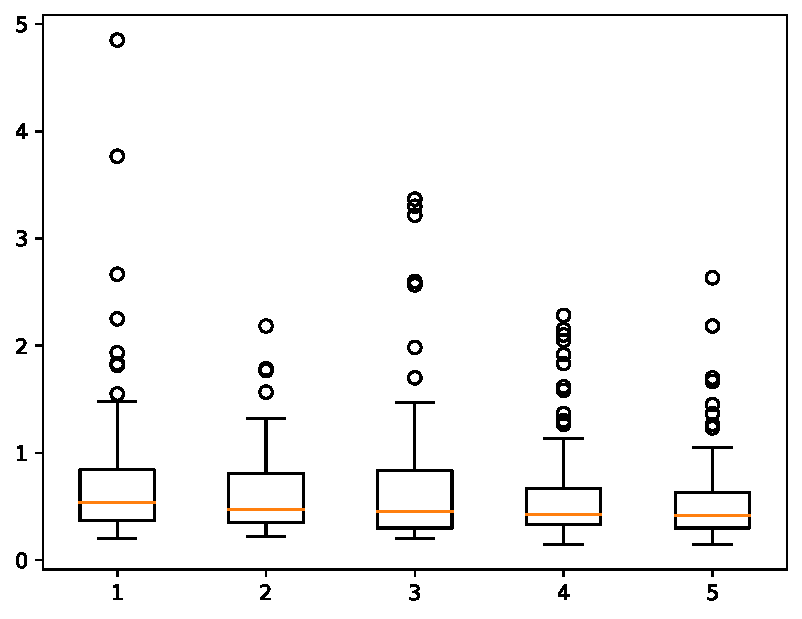
\includegraphics[scale=0.4]{images/homogeneity-test-for-thursday-hour-7.pdf}
            \caption{Boxplot.}
            \label{subfig:boxplot}
        \end{subfigure}
        \begin{subfigure}[b]{0.475\textwidth}   
            \centering 
            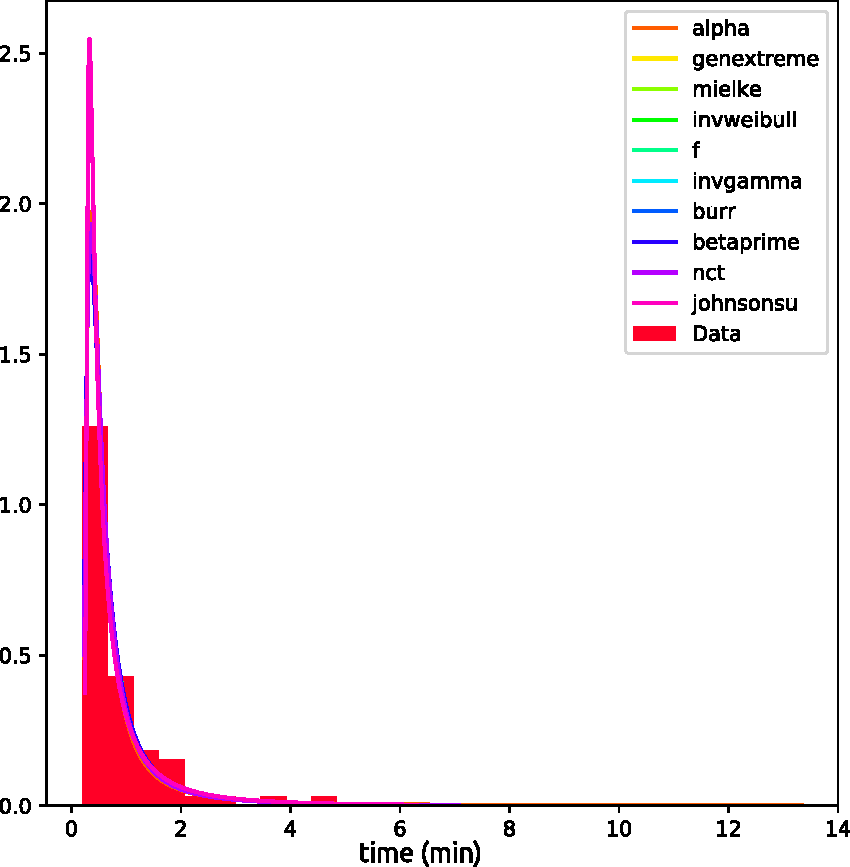
\includegraphics[scale=0.3]{images/fitting.pdf}
            \caption{Distribution fitting.}
            \label{subfig:dist}
        \end{subfigure}
        \caption{Data for Thursdays at 7 a.m.}
        \label{fig:thu7}
	\end{figure}
\end{frame}
